\documentclass[11pt]{revtex4-1}

\usepackage[colorlinks=true,urlcolor=blue]{hyperref}

\newcommand{\PRE}[1]{{#1}}
\newcommand{\secref}[1]{Sec.~\ref{sec:#1}}
\newcommand{\figref}[1]{Fig.~\ref{fig:#1}}
\newcommand{\tableref}[1]{Table~\ref{table:#1}}


\usepackage{epsfig}



\begin{document}

\title{ \PRE{\vspace*{1.5in}} Into the Cacophony -- Classification of
  Tweets on Twitter \PRE{\vspace*{0.3in}}}

\author{David Sanford}
\affiliation{DSI-SM03 \\General Assembly}

\date{March 2017}

\begin{abstract}
\PRE{\vspace*{.3in}} In this project I considered a classification
scheme for tweets on twitter.  I considered a data set of forty
thousand tweets, evenly split between unfiltered tweets and a sample
generated from a keyword filter using names of video game franchises.
I trained a set of machine learning estimators using half the data
set, resulting in cross-validation accuracies of between 75\% and 83\%
on the training set and 76\% for the best model on the validation set.
I also outline the possible methods for organizing topic-related
tweets into clusters based on genre or topic.
\end{abstract}

\maketitle



%\section{Introduction}
%\label{sec:introduction}



%In \secref{data}, I describe the data manipulation methods and data
%set used for the analysis.  In \secref{cleaning} I describe the data
%cleaning methods applied to the data set.  In \secref{lsa} I use a
%Latent Semantic Analisys pipeline to decompose the tweets for use in
%modeling.  In \secref{classification} I consider a binary
%classification of tweets between topic-related and unfiltered.

\section{Data Set}
\label{sec:data}

Data for this project was streamed from twitter using the twitter API
through the \href{http://pythonhosted.org/tweepy/}{\sc Tweepy} library
as an interfact in python.  Tweets were loaded into a
\href{http://www.mongodb.com/}{\sc Mongo} database running on a
\href{http://www.docker.com/}{\sc Docker} container.  Tweets loading
was performed in the notebook
\href{http://github.com/davidsanford/DSI_Capstone/blob/master/Tweet-Loading.ipynb}{Tweet-Loading.ipynb}.
Around three hundred thousand tweets were collected, but only two
hundred thousand were in english and a fraction of those were used due
to processing power constraints.  The tweets were collected in the
window of March 1-4, 2017.

For analysis, python was used with data held in the
\href{http://pandas.pydata.org/}{\sc Pandas} library.  Pre-processing
and machine learning were performed using
\href{http://scikit-learn.org/stable/}{\sc Scikit-Learn}.  Data was
pulled from the Mongo database through a spark intermediary database
using a
\href{http://spark.apache.org/docs/0.9.0/python-programming-guide.html}{\sc
  Pyspark} interface.  This was necessary due to memory constraints
relative to the size of the database, from which only a small subset
of the data was desired.

In terms of topic selection for classification, there are two apparent
options for generating a large set of topic-related tweets.  The first
is to generate a curated list of users who tweets exclusively about
that topic.  This approach is difficult, as most users with a large
volume of tweets will write off-topic tweets, which will contaminate
the data set.  Moreover, if the number of users chosen is too small
the word choice of the individual users themselves will also be baked
into the model, reducing classification effectiveness for unfiltered
tweets.

The method used here is to gather topic-related tweets based on a
series of keywords.  For this approach to be viable, the topic chosen
must have a sufficient number of keywords to produce a clean data set.
Several topics were considered for this project before video games,
including academic subjects, tabletop role-playing games, and tabletop
board games.  However, none of these subjects had sufficiently clean
sets of keywords on which to filter tweets.  Most video game
franchises, however, are unique words or combinations of words,
allowing for a large, relatively clean data set to be produced with a
wide variety keywords.

The list of 86 keywords below was used to filter topic-related tweets.

\begin{center}
\begin{tabular}{p{14cm}}
{\tiny Zelda, Tetris, Mario, Chrono Trigger, Street Fighter, Final
  Fantasy, Metroid, Half-Life, Resident Evil, Metal Gear, Castlevania,
  Pokemon, BioShock, SoulCalibur, StarCraft, Shadow of the Colossus,
  Doom, Diablo, World of Warcraft, Donkey Kong, Pac-Man, Halo, Deus
  Ex, Space Invaders, Sonic, Counter-Strike, Grim Fandango, Portal,
  Mass Effect, Last of Us, Star Fox, Mega Man, EarthBound, Prince of
  Persia, Call of Duty, Dark Souls, Perfect Dark, Ico, The Elder
  Scrolls, Skyrim, Morrowind, Silent Hill, Shenmue, Grand Theft Auto,
  Okami, Double Dragon, Red Dead, Galaga, Tomb Raider, Fallout,
  Uncharted, Assassin's Creed, Minecraft, Kingdom Hearts, Xenogears,
  Overwatch, Wii Sports, Wii Fit, The Sims, Terraria, Brain Age, Need
  for Speed, Lemmings, Madden NFL, Star Wars: Battlefront, Tom
  Clancy's, Duck Hunt, Splatoon, Super Smash, Dynasty Warriors,
  Monster Hunter, Kirby, Fire Emblem, Animal Crossing, God of War,
  Tekken, Garry's Mod, Myst, Angry Birds, Candy Crush, Fruit Ninja,
  Block Breaker, Doodle Jump, Space Invaders, Galaxian, Mortal Combat,
  Pong, Crysis}
\end{tabular}
\end{center}

\noindent The list was taken from the Wikipedia lists of
\href{http://en.wikipedia.org/wiki/List_of_video_games_considered_the_best}{well-rated}
and
\href{http://en.wikipedia.org/wiki/List_of_best-selling_video_games}{high-selling}
games.  Only key franchise words were used, and many older game names
were dropped due to likely irrelevance.  Franchise names that have
broader contexts, for instance ``Civilization'' and ``Battlefield''
were also excluded to avoid contaminating the sample.





\section{Data Cleaning}
\label{sec:cleaning}

Data cleaning is performed in the notebook
\href{http://github.com/davidsanford/DSI_Capstone/blob/master/Initial_Loading_and_Cleaning.ipynb}{Initial\_Loading\_and\_Cleaning.ipynb},
using methods from
\href{http://github.com/davidsanford/DSI_Capstone/blob/master/lib/tweet_cleaning.py}{lib/tweet\_cleaning.py}.
Tweets hashtags, username references, retweet tags, emojis, links, and
garbage strings containing letter/number combinations are all removed.
Male and female proper names and surnames are also removed if they are
within th 500 most popular names of their categoy based on
\href{http://catalog.data.gov/dataset/names-from-census-1990}{1990
  U.S. Census data}.

Strings from the keyword list are also removed based after the video
game tweets are categorized by keyword.  Only tweets containing a
single keyword are included in the ``video game'' data set, and only
tweets with no keywords are included in the ``unfiltered'' data set.
From these data sets, twenty thousand tweets from each are chosen and
divided evenly to produce equally-weighted training and validation
sets of twenty thousand tweets apiece.





\section{LSA Pre-Processing for Binary Classification}
\label{sec:lsa}

The cleaned training set from \secref{cleaning} must be processed
before it can be passed to classification methods.  For this purpose I
used a Latent Semantic Analsys (LSA) pipeline.  The relevant code is
included in the notebook
\href{http://github.com/davidsanford/DSI_Capstone/Binary_Classification_Model.ipynb}{Binary\_Classification\_Model.ipynb},
using methods from the library
\href{http://github.com/davidsanford/DSI_Capstone/lib/lsa.py}{lib/lsa.py}.
The cleaned text is first vectorized using TF-IDF vectorization, using
words appearing in between 0.1\% (100) and 50\% (5000) documents.
Stop words were left in the sample, as removing them resulted in over
10\% of the data set being reduced to empty sparse vectors.  With stop
words included, less than 5\% of the training and validation sets
were reduced to empty vectors.

The TF-IDF transformation resulted in 1172 features in sparse
matrices, which were then fed through a truncated SVD transformation.
The number of components kept was 200, which explained 56\% of the
total variance, as shown in \figref{explained_variance}.  While not
optimal, I judged this to be sufficient given the constraints in
processing power.

\begin{figure}[tbh]
  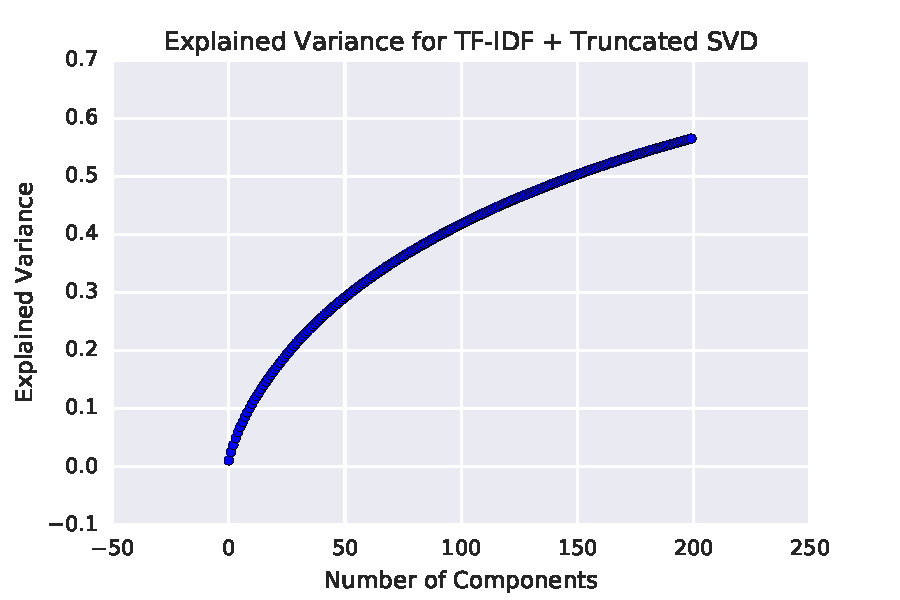
\includegraphics[width=0.7\textwidth]{variation.pdf}
  \caption{\emph{Figure 1: Explained Variance.}  Total explained
    variance by number of components included for TF-IDF + Truncated
    SVD}
  \label{fig:explained_variance}
\end{figure}





\section{Binary Classification}
\label{sec:classification}

Using the data sets generated through LSA in \secref{lsa}, binary
classification was performed using the six classification estimators
in \tableref{estimators}.  Due to processing limitation, only the
scikit-learn default parameters were used.  Training was performed on
70\% of the training set, using 5-fold cross-validation.  A test
accuracy was calculated using the remaining 30\% of the training set.

\begin{table}
  \begin{tabular}{|l|l|}
    \hline
    Estimator & Parameters \\
    \hline
    K-Nearest Neighbors & 5 neighbors, weighted by distance \\
    Logistic Regression & L2 regression with C = 1 \\
    SVC & RBF kernel, C = 1 \\
    Decision Tree & Gini impurity \\
    Random Forest & Gini impurity, 10 estimators \\
    Extra Trees & Gini impurity, 10 estimators \\
    \hline
  \end{tabular}
  \label{table:estimators}
  \caption{\emph{Table 1: Estimators and parameters.}  All parameters,
    both present and omitted, correspond to the scikit-learn
    defaults.}
\end{table}

The training and test accuracies for each estimator is shown in
\tableref{accuracies}.  The performance was reasonably similar for all
the estimators used and almost identical for the training and test
scores, ranging from 75\% to 83\% accuracy.  This suggests that the
correlations in the data are mostly linear, with variance resulting
from ``bleeding'' of the classes into one another rather than number
of dimensions rather than meaninful non-linear correlations.

\begin{table}
    \begin{tabular}{|l|l|l|}
      \hline
      Estimator & Train Accuracy & Test Accuracy \\
      \hline
      K-Nearest Neighbors & 0.783333 & 0.792444 \\
      Logistic Regression & 0.774190 & 0.781444 \\
      SVC & 0.822619 & 0.832889 \\
      Decision Tree & 0.744524 & 0.751778 \\
      Random Forest & 0.783048 & 0.792778 \\
      Extra Trees & 0.790571 & 0.794000 \\
      \hline
    \end{tabular}
  \label{table:accuracies}
  \caption{\emph{Table 2: Training accuracies.}  Training accuracy is
    the average over 5-fold cross-validation.  Test accuracy
    corresponds to the 30\% of the training set not used in
    cross-validation.}
\end{table}

This is supported by the results of a random forest grid scan over the
parameters given in \tableref{rfgrid}, which showed only marginal
improvement in performance.  The random forest model was chosen for
the grid search over the moderately better-performing SVC model due to
a shorter training time.

\begin{table}
    \begin{tabular}{|l|l|}
      \hline
      Parameter & Values \\
      \hline
      'criterion' & ['gini','entropy'] \\
      'n\_estimators' & [2,5,10,20] \\
      'max\_features' & [None, 'auto', 'sqrt','log2'] \\
      \hline
      Train Accuracy & 0.805905 \\
      Test Accuracy & 0.813 \\
      \hline
    \end{tabular}
    \label{table:rfgrid}
    \caption{\emph{Table 3: Random forest grid search parameters and
        scores.}  Training and testing accuracies are drawn from the
      same sets as in \tableref{accuracies}}
\end{table}

Using the SVC estimator, the metrics in \tableref{validation} were
calculated on the validation set.  The accuracy was moderately lower
than the training accuracy, but still reasonably at 76\%.  More
interestingly, the precision had a relatively high value of 90\%,
indicating that the identified sample of video game related tweets
should be relatively clean.  Recall, however, is only 0.6, indicating
that only 60\% video game related tweets in an unfiltered stream will
be tagged.   

\begin{table}
      \begin{tabular}{|l|l|l|l|l|}
        \hline
        Model & Accuracy & Precision & Recall & F1-Score \\
        \hline
        SVC & 0.76 & 0.90 & 0.60 & 0.72 \\
        \hline
      \end{tabular}
    \label{table:validation}
    \caption{\emph{Table : Metrics on validation set.}  All metrics
      used the entire validation set with the appropriate
      transformation applied to the raw data.}
\end{table}

This effect is even more pronounce in the ROC curve shown in
\figref{roc_curve}.  The false positive rate falls to less than 10\%
with the true positive rate still over 40\%, so the model can easily
be optimized for a low false positive rate while retaining a
non-negligible true positive rate.  However, achieving a high true
positive rate requires acceptance of a significant false positive
rate.  A true positive rate of 80\% requires a false positive rate of
40\%, and a true positive rate of 90\% requires a false positive rate
of 90\%.

\begin{figure}[tbh]
  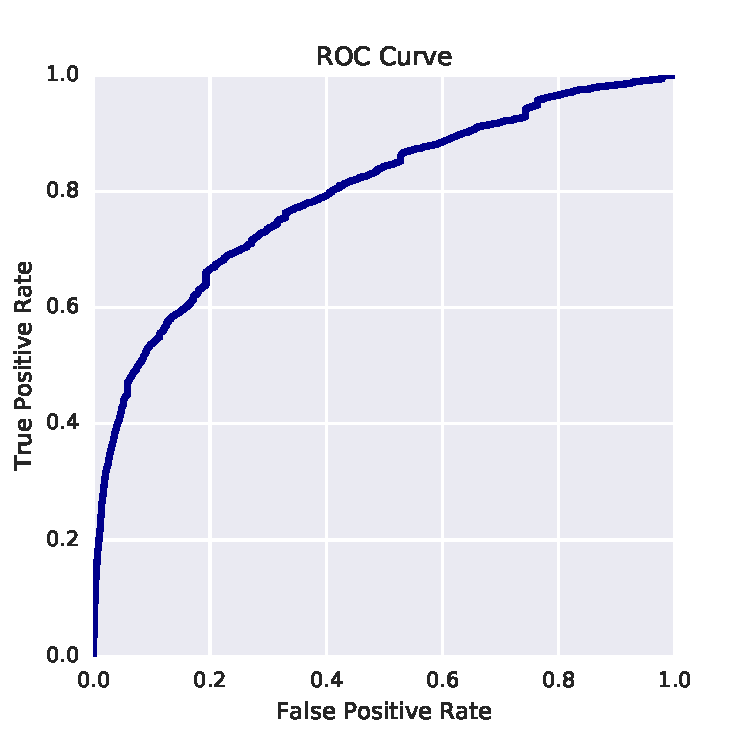
\includegraphics[width=0.7\textwidth]{ROC_Curve.pdf}
  \caption{\emph{Figure 2: ROC Curve.}  Results of variation in the
    threshold for the best-performing SVC model on the validation
    set.}
  \label{fig:roc_curve}
\end{figure}





\section{Classification Model Performance and Improvement}
\label{sec:analysis}

The binary classification model examined here has a reasonable
accuracy of around 75\%, at least on the validation set.  Further
validation using a separate set of brand keywords is advisable, as the
estimator may be overfit on brand-specific terms, and its true
peformance for video games of all stripes may be lower.  Consideration
of a hand-selected set of tweets with manual classification for
ultimate validation may also be desireable.  On the positive side,
this methodology should function for any topic with sufficiently
distinct keywords, and it would be interesting to apply it to a corpus
fo tweets selected using one of the terms already identified as
ambiguous to judge performance out of the box.

Real gains in performance, however, likely require more careful
curation of the origin data set and iterations on the analysis
framework.  Beyond the first step of accessing more processing power,
some method of bootstrapping might provide better results.  Many
tweets are short, or even empty after keywords and stop words are
removed, making them non-ideal for training.  A procedure of
concatenating random groups of the strings to artificially generate
longer individual documents might improve performance.  Alternatively,
based upon the ultimate use case, a simple cut to remove excessively
short and low-information tweets might be appropriate.

\begin{table}
  \begin{tabular}{|l|l|l|}
    \hline
    Keyword & Percentage & Total \\
    \hline
    Zelda & 35.056 & 8764 \\
    Overwatch & 11.116 & 2779 \\
    Pokemon & 7.452 & 1863 \\
    Minecraft & 5.260 & 1315 \\
    Mario & 5.196 & 1299 \\
    Halo & 3.072 & 768 \\
    Sonic & 3.052 & 763 \\
    Mass Effect & 2.980 & 745 \\
    Resident Evil & 2.592 & 648 \\
    Call of Duty & 2.108 & 527 \\
    \hline
  \end{tabular}
  \caption{\emph{Prevalence of Keywords.}  Top ten most prevalent
    keywords and the percentage of the training set that they
    compose.}
  \label{table:prevalence}
\end{table}

Balancing the sub-classes and genres might also improve results.  As
shown in \tableref{prevalence}, the relative appearance rate of
various brands in the data set very weighted, with Zelda in particular
appearing three times as much as the next most prevalent term
(probably due to the time period in which the tweets were collected).
Beyond this, balancing the number of tweets in the training sample by
game genres might improve general results.  That said, it is
conceivable that some sub-topics are simply easier to classify than
others -- fantasy and science fiction games, for example, have more
specialized vocabulary associated with them than those set in the real
world.

\section{Genre/Topic Clustering}
\label{sec:clustering}

Building upon binary classification, it would be desireable to
classify tweets within sub-categories once they are identified as
video game tweets.  This could be an attempt to identify as related to
a particular brand, to identify the genre of the game being discussed,
or identify the topics being addressed in the tweet.  The first use
case likely reduces to keyword searches on brand-specific words, so
the latter two possibilities are more interesting.

Neither avenue of inquiry has yet yielded results, so I will sketch
possible approaches, based on code in
\href{https://github.com/davidsanford/DSI_Capstone/Video_Game_Sub-Categorization.ipynb}{Video\_Game\_Sub-Categorization.ipynb}.
Genre identification requires applying clustering algorithm to tweets
processed through LSA, then attempting to identify genres based on the
prevalence of various games within each cluster.  Another approach
might be to generate a corpus for each keyword out of all tweets
associated with that keyword, then cluster those documents.  Either of
these approaches is hampered by the relative prevalence of tweets with
particular keywords in the data set, as discussed above and shown in
\tableref{prevalence}.  A more uniform selection of keywords through
more careful curation is probably necessary for these purposes.




Topic modeling would instead focus on broad topics being discussed by
twitter users, spanning different games and genres.  Indentifying
these topics would involve applying Latent Dirichlet Allocation (LDA)
to the corpus and identifying key terms in each topic.  An initial
pass produced a grouping of naively unrelated terms.  If topic
modeling is appropriate for this corpus a significant amount of
iteration in removing meaningless words would likely be necessary, and
the technique may not be appropriate for the diversity of grammar
present in tweets from a multitude of different users.



\section{Conclusion}
\label{sec:conclusion}

In this report I described a project to classify tweets on twitter by
topic, using a sample drawn from a set of selected keywords over a
large number of users.  I fit a binary classification model which
demonstrates 75\% classification accuracy, and discussed possible
methods to improve its performance in the future.  I also discussed
the initial stages and possible extension of two separate
sub-classification schemes to extract further information from
topic-related tweets.

The techniques described here, while simplistic, are broadly
applicable.  Going beyond keyword filtering to topic classification on
a corpus is useful to discriminate any text on the internet, from
comment threads and discussion boards to news stories and long blog
posts.  This identification could be used to select pages for an end
user by a search engine, identify relevant documents for internal
company use, or even select a clean set of documents for deeper NLP
analyses.

\end{document}
